\documentclass[t]{beamer}
\mode<presentation>

\setbeamertemplate{itemize items}[circle]
\usepackage{palatino}
\usepackage{apalike}
\usepackage{graphicx} % Required for including images
\graphicspath{{figures/}} % Location of the graphics files
\usepackage{booktabs} % Top and bottom rules for table
\usepackage[font=small,labelfont=bf]{caption} % Required for specifying captions to tables and figures
\usepackage{wrapfig} % Allows wrapping text around tables and figures
\usepackage{lipsum,adjustbox}
\usepackage[absolute,overlay]{textpos}
\usepackage{url}
\usepackage{lmodern}
\usepackage{amsmath}
\usepackage{amsfonts}
\usepackage{color}
\usepackage{array}
\usepackage{multirow}
\usepackage{multicol}
\usepackage{tikz}
\usepackage{tikz-dependency}
\usepackage{neuralnetwork}
\usetikzlibrary{arrows.meta,graphs,graphs.standard,graphdrawing,quotes,shapes}
\usegdlibrary{layered,trees}
\tikzset{
  invisible/.style={opacity=0},
  visible on/.style={alt={#1{}{invisible}}},
  alt/.code args={<#1>#2#3}{%
    \alt<#1>{\pgfkeysalso{#2}}{\pgfkeysalso{#3}} % \pgfkeysalso doesn't change the path
  },
}
\captionsetup{labelformat=empty}
\newcommand{\parser}[1]{TUPA\textsubscript{#1}}

\makeatletter
\pgfdeclareshape{vector}{
	  \inheritsavedanchors[from={rectangle}]
	  \inheritbackgroundpath[from={rectangle}]
	  \inheritanchorborder[from={rectangle}]
	  \foreach \x in {center,north east,north west,north,south,south east,south west,east,west}{
	    \inheritanchor[from={rectangle}]{\x}
	  }

    \backgroundpath{
      \pgftransformshift{\pgfpoint{-16pt}{-4pt}}
		  \draw[rounded corners=2pt] (0,0) rectangle (32pt,8pt);
    }

    \beforebackgroundpath{
      \draw[step=8pt,help lines,-] (8pt,.1pt) grid (24pt,7.9pt);
    }
}
\makeatother


\begin{document}


\title[A Transition-Based DAG Parser for UCCA]{A Transition-Based Directed Acyclic Graph Parser for Universal Conceptual Cognitive Annotation}
\author{Daniel Hershcovich, Omri Abend and Ari Rappoport}
\institute[]{
\includegraphics[width=.08\pagewidth]{huji_logo.jpg}

\includegraphics[width=.3\pagewidth]{huji_banner.png}}
\date{Technion \\ June 29, 2017}
%\date{ACL 2017}

\begin{frame}
\titlepage
\end{frame}


%----------------------------------------------------------------------------------------

%%%%%%%%%%%%%%%%%%%%%%%%%%%%%%%%%%%%%%%%%%%%%%%%%%%%%%%%%%%%%%%%%%%%%%%%%%%%%%%%%%%%
\section{Introduction}

\begin{frame}
\frametitle{Dependency Parsing}
\begin{itemize}
	\item Graph representation of syntactic structure.
	\item Bilexical tree: edges are only between tokens.
	\item Fast and accurate parsers (e.g. \textit{transition-based}).
\end{itemize}
\vfill
\begin{adjustbox}{frame,center}
\begin{dependency}
	\begin{deptext}[column sep=1.5em,ampersand replacement=\^,font=\rmfamily]
	After \^ graduation \^ , \^ Joe \^ moved \^ to \^ Paris \\
	\end{deptext}
	\deproot{5}{root}
	\depedge{2}{1}{case}
	\depedge{5}{2}{nmod}
	\depedge{5}{3}{punct}
	\depedge{5}{4}{nsubj}
	\depedge{7}{6}{case}
	\depedge{5}{7}{nmod}
\end{dependency}
\end{adjustbox}

\pause
Non-projectivity (discontinuity) is a challenge \cite{nivre2009non}.
\begin{adjustbox}{scale=.8,frame,center}
\begin{dependency}
	\begin{deptext}[column sep=1.2em,ampersand replacement=\^,font=\rmfamily]
	A \^ hearing \^ is \^ scheduled \^ on \^ the \^ issue \^ today \\
	\end{deptext}
	\deproot{4}{root}
	\depedge{2}{1}{det}
	\depedge{4}{2}{nsubj:pass}
	\depedge{4}{3}{aux:pass}
	\depedge{7}{5}{case}
	\depedge{7}{6}{det}
	\depedge[edge start x offset=-6pt,red]{2}{7}{nmod}
	\depedge[edge slant=6pt]{4}{8}{nmod:tmod}
\end{dependency}
\end{adjustbox}
\end{frame}

\begin{frame}
\frametitle{Semantic Dependency Parsing}
\begin{itemize}
	\item Representation of predicate-argument relationships.
	\item Bilexical graph: allows reentrancy (and discontinuity).
	\item Various formalisms \cite{oepen2015semeval}.
\end{itemize}
\vfill

\begin{adjustbox}{scale=.9,frame,center}
\begin{dependency}
	\begin{deptext}[column sep=1.5em,ampersand replacement=\^,font=\rmfamily]
	After \^ graduation \^ , \^ Joe \^ moved \^ to \^ Paris \\
	\end{deptext}
	\deproot[edge style={red}]{5}{top}
	\depedge{1}{2}{ARG2}
	\depedge[edge slant=10pt,red]{1}{5}{ARG1}
	\depedge{5}{4}{ARG1}
	\depedge[red]{6}{5}{ARG1}
	\depedge{6}{7}{ARG2}
\end{dependency}
\end{adjustbox}
\captionof{figure}{DELPH-IN MRS-derived bi-lexical dependencies (DM).}

\pause
\begin{adjustbox}{scale=.9,frame,center}
\begin{dependency}
	\begin{deptext}[column sep=1.5em,ampersand replacement=\^,font=\rmfamily]
	After \^ graduation \^ , \^ Joe \^ moved \^ to \^ Paris \\
	\end{deptext}
	\deproot{5}{top}
	\depedge{5}{2}{TWHEN}
	\depedge{5}{4}{ACT-arg}
	\depedge{5}{7}{DIR3-arg}
\end{dependency}
\end{adjustbox}
\captionof{figure}{Prague Dependency Treebank tectogrammatical layer (PSD).}
\end{frame}
%%%%%%%%%%%%%%%%%%%%%%%%%%%%%%%%%%%%%%%%%%%%%%%%%%%%%%%%%%%%%%%%%%%%%%%%%%%%%%%%%%%%


\section{Universal Conceptual Cognitive Annotation}

\begin{frame}
\frametitle{Universal Conceptual Cognitive Annotation (UCCA)}
\begin{tikzpicture}[level distance=25mm, sibling distance=23mm, ->,
    every circle node/.append style={fill=black},
    every node/.append style={font=\rmfamily}]
  \node (ROOT) [circle] {}
    child {node (After) {After} edge from parent node[left] {$L$}}
    child {node (graduation) [circle] {}
    {
      child {node {graduation} edge from parent node[left] {$P$}}
    } edge from parent node[left] {$H$} }
    child {node {,} edge from parent node[right] {$U$}}
    child {node (moved) [circle] {}
    {
      child {node (Joe) {Joe} edge from parent node[left] {$A$}}
      child {node {moved} edge from parent node[left] {$P$}}
      child {node [circle] {}
      {
        child {node {to} edge from parent node[left] {$R$}}
        child {node {Paris} edge from parent node[right] {$C$}}
      } edge from parent node[right] {$A$} }
    } edge from parent node[right] {$H$} }
    ;
  \draw[dashed,->] (graduation) to node [auto] {$A$} (Joe);
  \node at (5.6,-.3) {\Large ----- primary edge};
  \node at (5.6,-1.3) {\Large - - - remote edge};
\end{tikzpicture}
\begin{wraptable}{l}{8cm}
  \vspace{-27mm}
  \hspace{14mm} After graduation, Joe moved to Paris
  \begin{adjustbox}{margin=1mm,frame}
  \scalebox{.7}{
  \begin{tabular}{c>{\small\it}l|c>{\small\it}l|c>{\small\it}l}
	  $P$ & process &
	  $S$ & state &
	  $A$ & participant \\
	  $L$ & linker &
	  $H$ & linked scene &
	  $C$ & center \\
	  $E$ & elaborator &
	  $D$ & adverbial &
	  $R$ & relator \\
	  $N$ & connector &
	  $U$ & punctuation &
	  $F$ & function \\
	  $G$ & ground
  \end{tabular}
  }
  \end{adjustbox}
\end{wraptable}
\end{frame}

\begin{frame}
\frametitle{The UCCA Semantic Representation Scheme}
Cross-linguistically applicable \cite{abend2013universal}.
Stable in translation \cite{sulem2015conceptual}.
\vfill
\begin{adjustbox}{center}
  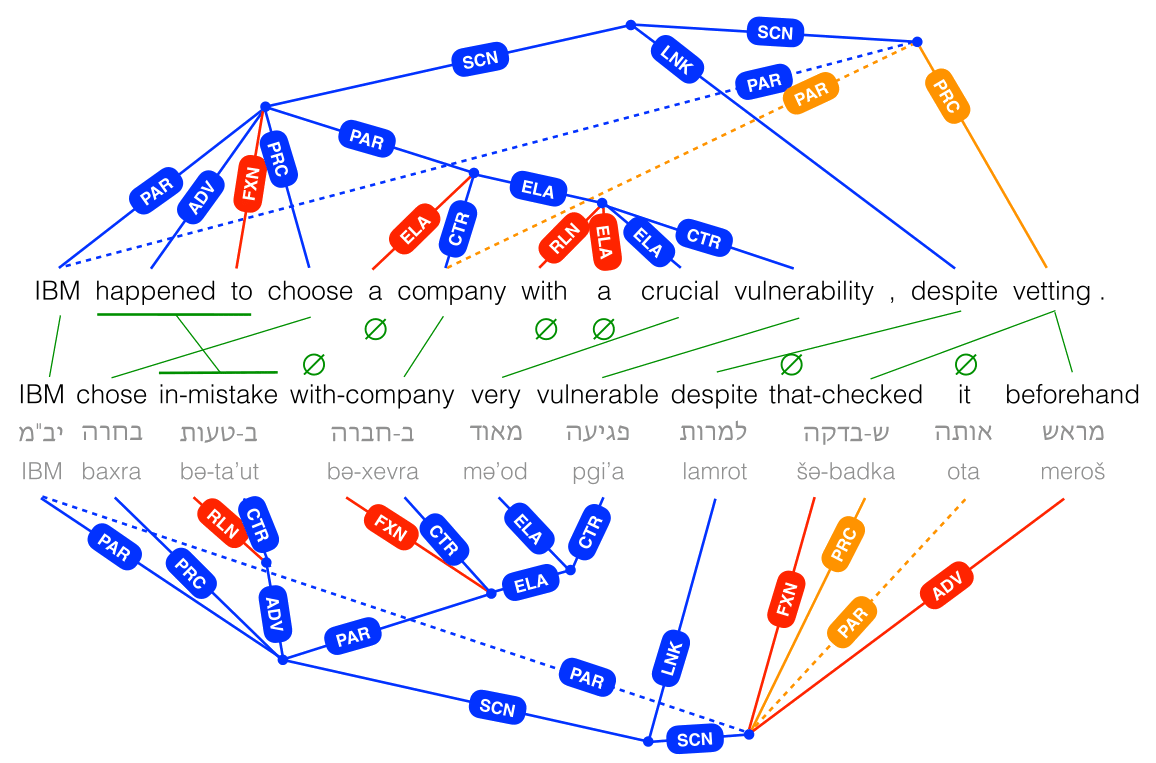
\includegraphics[width=\textwidth,height=\textheight,keepaspectratio]{crosslinguistic.png}
\end{adjustbox}
\end{frame}

\begin{frame}
\frametitle{UCCAApp}
Rapid and intuitive annotation interface \cite{abend2017uccaapp}.
Usable by non-experts.
\footnotesize\url{http://ucca-demo.cs.huji.ac.il}
\vfill
\begin{adjustbox}{center}
  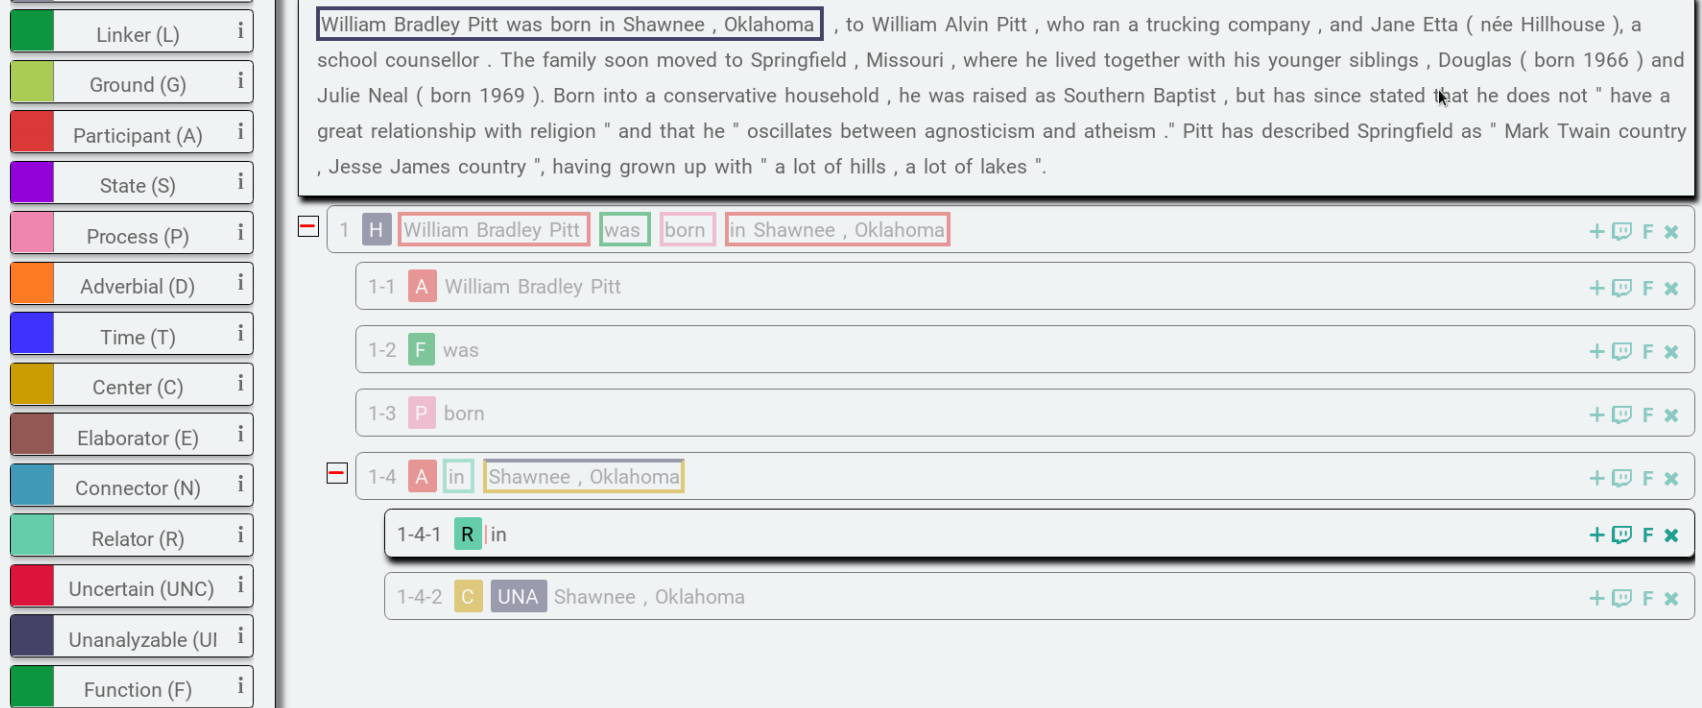
\includegraphics[width=\pagewidth,height=\textheight,keepaspectratio]{uccaapp.png}
\end{adjustbox}
\end{frame}

\begin{frame}
\frametitle{HUME}
UCCA facilitates semantics-based human evaluation of machine translation \cite{birch2016hume}.
\footnotesize\url{http://ucca.cs.huji.ac.il/mteval}
\vfill
\begin{adjustbox}{center}
  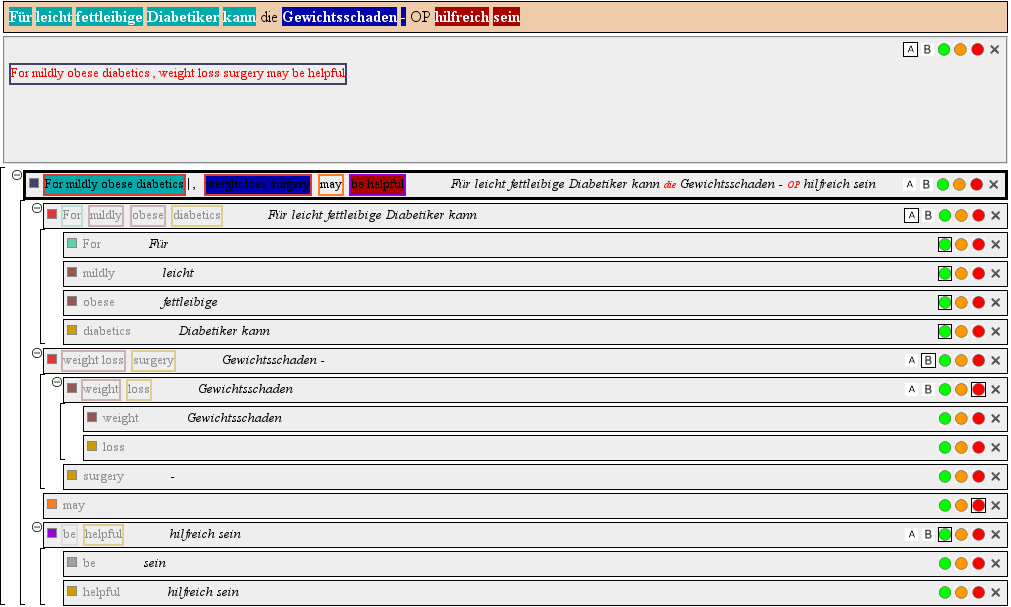
\includegraphics[width=\pagewidth,height=\textheight,keepaspectratio]{hume.png}
\end{adjustbox}
\end{frame}

\begin{frame}
\frametitle{Graph Structure}
UCCA forms a directed acyclic graph (DAG). Tokens are terminals.
Its semantic distinctions \cite{abend2017the} require:
\begin{enumerate}
\item<1-> \color{blue} Non-terminal nodes
\item<2-> \color{orange} Reentrancy
\item<3-> \color{red} Discontinuity
\end{enumerate}
\centering

\vfill
 \newcommand*\reecol{}
 \newcommand*\reewid{}
 \only<2->{\renewcommand*\reecol{orange}}
 \only<2->{\renewcommand*\reewid{very thick}}
 \newcommand*\discol{}
 \newcommand*\diswid{}
 \only<3->{\renewcommand*\discol{red}}
 \only<3->{\renewcommand*\diswid{very thick}}
  \begin{tikzpicture}[level distance=12mm, sibling distance=2cm, ->,
      every node/.append style={font=\rmfamily}]
    \node (ROOT) [fill=blue, circle] {}
      child {node (You) {You} edge from parent node[left] {\scriptsize $A$}}
      child {node {want} edge from parent node[left] {\scriptsize $P$}}
      child {node (totakealongbath) [fill=blue, circle] {}
      {
        child {node {to} edge from parent node[left] {\scriptsize $F$}}
        child {node (takeabath) [fill=blue, circle] {}
        {
          child {node {take} edge from parent node[right] {\scriptsize $C$}}
          child {node {a} edge from parent node[right] {\scriptsize $F$}}
          child {node (long) {long} edge from parent[white]}
          child {node {bath} edge from parent node[right] {\scriptsize $C$}}
        } edge from parent node[right] {\scriptsize $P$} }
      } edge from parent node[left] {\scriptsize $A$} }
      ;
    \draw[bend left,dashed,->,\reecol,\reewid] (takeabath) to node [auto] {\scriptsize $A$} (You);
    \draw[bend left,->,\discol,\diswid] (totakealongbath) to node [auto] {\scriptsize $D$} (long);
  	\node at (5.6,-.3) {\small ----- primary edge};
  	\node at (5.6,-.8) {\small - - - remote edge};
  \end{tikzpicture}
\vfill
You want to take a long bath
\end{frame}



\section{Transition-based UCCA Parsing}

\begin{frame}
\frametitle{Transition-Based Parsing}
\begin{itemize}
 \item Parse text $w_1 \ldots w_n$ to graph $G=(V,E,\ell)$ incrementally.
 \item Classifier determines transition to apply at each step.
 \item Trained by an oracle based on gold-standard graph.
\end{itemize}
\pause
Initial state:
\begin{tikzpicture}[every node/.append style={font=\rmfamily}, circle]
	\draw[xstep=1cm,ystep=5mm,color=gray] (-0.01,0) grid (1,.5);
	\node[anchor=west] at (-0.1,1.00)     {stack};
	\node[fill=black] at (0.5,0.25) {};
	\draw[xstep=1cm,ystep=5mm,color=gray] (3,0) grid (10,.5);
	\node[anchor=west] at (8.9,1.00) {buffer};
	\node[anchor=west] at (3,0.25) {\small You};
	\node[anchor=west] at (4,0.25) {\small want};
	\node[anchor=west] at (5,0.25) {\small to};
	\node[anchor=west] at (6,0.25) {\small take};
	\node[anchor=west] at (7,0.25) {\small a};
	\node[anchor=west] at (8,0.25) {\small long};
	\node[anchor=west] at (9,0.25) {\small bath};
\end{tikzpicture}

\vfill
\pause
\parser{} transitions:

\vfill
\{\textsc{Shift, Reduce, Node$_X$, Left-Edge$_X$, Right-Edge$_X$,}\\
\hspace{5mm}\textsc{Left-Remote$_X$, Right-Remote$_X$, Swap, Finish}\}

\vfill
Support non-terminal nodes, reentrancy and discontinuity.
\end{frame}

\begin{frame}
\frametitle{Transition-Based UCCA Parsing}
$\Rightarrow$\textsc{
\only<1>{Shift}\only<2>{Right-Edge\textsubscript A}\only<3>{Shift}\only<4>{Swap}\only<5>{Right-Edge\textsubscript P}\only<6>{Reduce}\only<7>{Shift}\only<8>{Shift}\only<9>{Node\textsubscript F}\only<10>{Reduce}\only<11>{Shift}\only<12>{Shift}\only<13>{Node\textsubscript C}\only<14>{Reduce}\only<15>{Shift}\only<16>{Right-Edge\textsubscript P}\only<17>{Shift}\only<18>{Right-Edge\textsubscript F}\only<19>{Reduce}\only<20>{Shift}\only<21>{Swap}\only<22>{Right-Edge\textsubscript D}\only<23>{Reduce}\only<24>{Swap}\only<25>{Right-Edge\textsubscript A}\only<26>{Reduce}\only<27>{Reduce}\only<28>{Shift}\only<29>{Shift}\only<30>{Left-Remote\textsubscript A}\only<31>{Shift}\only<32>{Right-Edge\textsubscript C}\only<33>{Finish}
}
\vfill
\begin{tikzpicture}[every node/.append style={font=\rmfamily}]
	\only<27>\draw[xstep=1mm,ystep=5mm,color=gray] (-0.01,0) grid (0.1,.5);
	\only<6,26,28>\draw[xstep=1cm,ystep=5mm,color=gray] (-0.01,0) grid (1,.5);
	\only<-2,4-5,7,10,24-25,29-30>\draw[xstep=1cm,ystep=5mm,color=gray] (-0.01,0) grid (2,.5);
	\only<3,8-9,11,14,23,31->\draw[xstep=1cm,ystep=5mm,color=gray] (-0.01,0) grid (3,.5);
	\only<12-13,15-16,19,21-22>\draw[xstep=1cm,ystep=5mm,color=gray] (-0.01,0) grid (4,.5);
	\only<17-18,20>\draw[xstep=1cm,ystep=5mm,color=gray] (-0.01,0) grid (5,.5);
	\node[anchor=west] at (-0.1,1.00){stack};
	\only<-26>\node[fill=black, circle] at (0.5,0.25) {};
	\only<24-25> \node[fill=blue, circle] at (1.5,0.25) {};
	\only<11-23> \node[fill=blue, circle] at (2.5,0.25) {};
	\only<29-> \node[fill=red, circle] at (1.5,0.25) {};
	\only<15-20> \node[fill=red, circle] at (3.5,0.25) {};
	\only<28-> \node[anchor=west] at (0,0.25) {\small You};
	\only<1-3,7-23> \node[anchor=west] at (1,0.25) {\small You};
	\only<4-5> \node[anchor=west] at (1,0.25) {\small want};
	\only<3>   \node[anchor=west] at (2,0.25) {\small want};
	\only<8-9>  \node[anchor=west] at (2,0.25) {\small to};
	\only<12-13> \node[anchor=west] at (3,0.25) {\small take};
	\only<17-18> \node[anchor=west] at (4,0.25) {\small a};
	\only<20> \node[anchor=west] at (4,0.25) {\small long};
	\only<21-22> \node[anchor=west] at (3,0.25) {\small long};
	\only<31-> \node[anchor=west] at (2,0.25) {\small bath};
	\only<-2,4-5>\draw[xstep=1cm,ystep=5mm,color=gray] (4,0) grid (10,.5);
	\only<3,5-7,9-10>\draw[xstep=1cm,ystep=5mm,color=gray] (5,0) grid (10,.5);
	\only<8,11,13-14>\draw[xstep=1cm,ystep=5mm,color=gray] (6,0) grid (10,.5);
	\only<12,15-16,24-27>\draw[xstep=1cm,ystep=5mm,color=gray] (7,0) grid (10,.5);
	\only<17-19,21-23,28>\draw[xstep=1cm,ystep=5mm,color=gray] (8,0) grid (10,.5);
	\only<20,29-30>\draw[xstep=1cm,ystep=5mm,color=gray] (9,0) grid (10,.5);
	\only<31->\draw[xstep=1mm,ystep=5mm,color=gray] (9.89,0) grid (10,.5);
	\node[anchor=west] at (8.9,1) {buffer};
	\only<9-10> \node[fill=blue, circle] at (5.5,0.25) {};
	\only<13-14> \node[fill=red, circle] at (6.5,0.25) {};
	\only<21-28> \node[fill=red, circle] at (8.5,0.25) {};
	\only<4-5> \node[anchor=west] at (4,0.25) {\small You};
	\only<24-27> \node[anchor=west] at (7,0.25) {\small You};
	\only<-2>  \node[anchor=west] at (4,0.25) {\small want};
	\only<-7> \node[anchor=west] at (5,0.25) {\small to};
	\only<-11> \node[anchor=west] at (6,0.25) {\small take};
	\only<-16> \node[anchor=west] at (7,0.25) {\small a};
	\only<-19> \node[anchor=west] at (8,0.25) {\small long};
	\only<-30> \node[anchor=west] at (9,0.25) {\small bath};
\end{tikzpicture}
\vfill
\fbox{
\begin{tikzpicture}[level distance=15mm, sibling distance=2cm, ->,
    every node/.append style={font=\rmfamily}]
	\node[anchor=west] at (0,0) {graph};
    \node(ROOT)[fill=black, circle, visible on=<1->] at (3,0) {}
      child [visible on=<2->] {node (You) {You} edge from parent node [left] {\scriptsize $A$}}
      child [visible on=<5->] {node {want} edge from parent node [left] {\scriptsize $P$}}
      child [visible on=<9->] {node (totakealongbath) [fill=blue, circle] {}
      {
        child [visible on=<9->] {node {to} edge from parent node [left] {\scriptsize $F$}}
        child [visible on=<13->] {node (takeabath) [fill=red, circle] {}
        {
          child [visible on=<13->] {node {take} edge from parent node [right] {\scriptsize $C$}}
          child [visible on=<18->] {node {a} edge from parent node [right] {\scriptsize $F$}}
          child [visible on=<22->] {node (long) {long} edge from parent [draw=none]}
          child [visible on=<32->] {node {bath} edge from parent node [right] {\scriptsize $C$}}
        } edge from parent [draw=none]}
      } edge from parent [draw=none]}
      ;
    \draw[visible on=<16->] (totakealongbath) to node [left] {\scriptsize $P$} (takeabath);
    \draw[visible on=<25->] (ROOT) to node [left] {\scriptsize $A$} (totakealongbath);
    \draw[bend left,dashed, visible on=<30->] (takeabath) to node [auto] {\scriptsize $A$} (You);
    \draw[bend left, visible on=<22->] (totakealongbath) to node [auto] {\scriptsize $D$} (long);
\end{tikzpicture}}
\end{frame}


%%%%%%%%%%%%%%%%%%%%%%%%%%%%%%%%%%%%%%%%%%%%%%%%%%%%%%%%%%%%%%%%%%%%%%%%%%%%%%%%%%%%
\section{Deep Learning for NLP}

\begin{frame}
\frametitle{Word Embeddings}
Represent discrete features by dense vectors \cite{goldberg2016primer}.
\vfill
\begin{adjustbox}{center}
  \includegraphics[width=\textwidth,height=\textheight,keepaspectratio]{feats.png}
\end{adjustbox}
\end{frame}

\begin{frame}[fragile]
\frametitle{Feed-Forward Neural Network (MLP)}
Learns representation and classification by optimizing weights.
\vfill
\begin{adjustbox}{center,scale=.9}
	\begin{neuralnetwork}[height=4,style={rotate=90},layertitleheight=5.5em,toprow=true]
		\newcommand{\nodetextclear}[2]{}
		\newcommand{\nodetextx}[2]{$x_#2$}
		\newcommand{\nodetexty}[2]{$y_#2$}
		\newcommand{\nodetexts}[2]{$\int$}
		\inputlayer[count=4, bias=false, title=Input layer, text=\nodetextx]
		\hiddenlayer[count=6, bias=false, title=Hidden layer, text=\nodetexts] \linklayers
		\hiddenlayer[count=5, bias=false, title=Hidden layer, text=\nodetexts] \linklayers
		\outputlayer[count=3, title=Output layer, text=\nodetexty] \linklayers
	\end{neuralnetwork}
\end{adjustbox}
\end{frame}

\begin{frame}
\frametitle{Recurrent Neural Network (RNN)}
Applied to sequences, updates state given input and previous state.
\vfill
\begin{adjustbox}{center}
  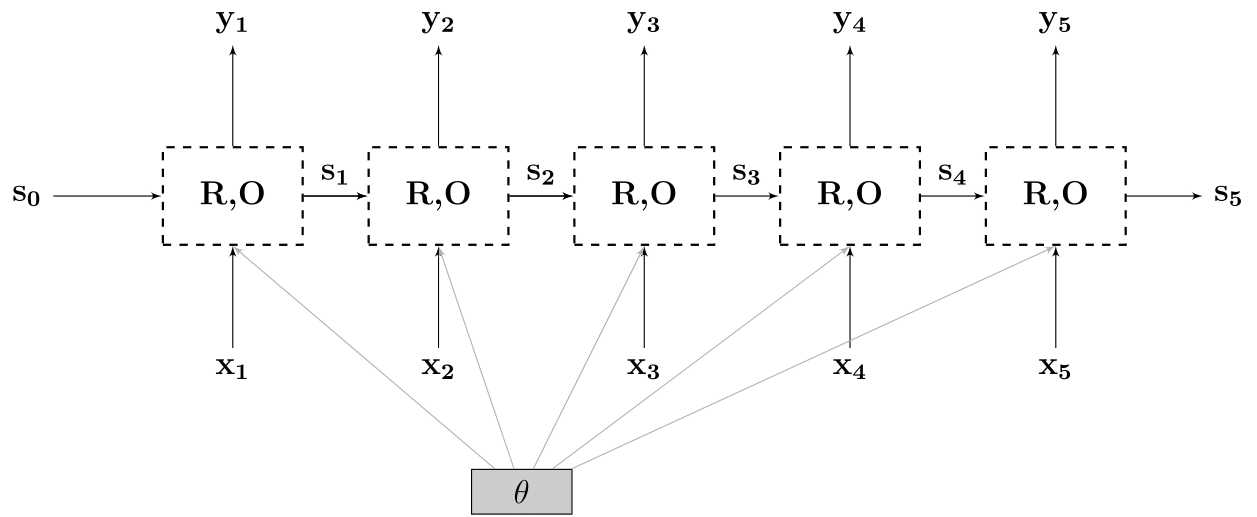
\includegraphics[width=\textwidth,height=\textheight,keepaspectratio]{rnn-unrolled.png}
\end{adjustbox}
\end{frame}

\begin{frame}
\frametitle{Long Short-Term Memory (LSTM)}
Memory cell to avoid vanishing gradients in RNNs.
\vfill
\begin{adjustbox}{center}
	\begin{tikzpicture}[
		    prod/.style={circle, draw, inner sep=0pt},
		    ct/.style={circle, draw, inner sep=5pt, ultra thick, minimum width=10mm},
		    ft/.style={circle, draw, minimum width=8mm, inner sep=1pt},
		    filter/.style={circle, draw, minimum width=7mm, inner sep=1pt, path picture={\draw[thick, rounded corners] (path picture bounding box.center)--++(65:2mm)--++(0:1mm);
		    \draw[thick, rounded corners] (path picture bounding box.center)--++(245:2mm)--++(180:1mm);}},
		    mylabel/.style={font=\scriptsize\sffamily},
		    >=LaTeX
		    ]
		\node[ct, label={[mylabel]Cell}] (ct) {$c_t$};
		\node[filter, right=of ct] (int1) {};
		\node[prod, right=of int1] (x1) {$\times$}; 
		\node[right=of x1] (ht) {$h_t$};
		\node[prod, left=of ct] (x2) {$\times$}; 
		\node[filter, left=of x2] (int2) {};
		\node[prod, below=5mm of ct] (x3) {$\times$}; 
		\node[ft, below=5mm of x3, label={[mylabel]right:Forget Gate}] (ft) {$f_t$};
		\node[ft, above=of x2, label={[mylabel]left:Input Gate}] (it) {$i_t$};
		\node[ft, above=of x1, label={[mylabel]left:Output Gate}] (ot) {$o_t$};
		\foreach \i/\j in {int2/x2, x2/ct, ct/int1, int1/x1,
		            x1/ht, it/x2, ct/it, ct/ot, ot/x1, ft/x3}
		    \draw[->] (\i)--(\j);
		\draw[->] (ct) to[bend right=45] (ft);
		\draw[->] (ct) to[bend right=30] (x3);
		\draw[->] (x3) to[bend right=30] (ct);
		\node[fit=(int2) (it) (ot) (ft), draw, inner sep=0pt] (fit) {};
		\draw[<-] (fit.west|-int2) coordinate (aux)--++(180:7mm) node[left]{$x_t$};
		\draw[<-] ([yshift=1mm]aux)--++(135:7mm);
		\draw[<-] ([yshift=-1mm]aux)--++(-135:7mm);
		\draw[<-] (fit.north-|it) coordinate (aux)--++(90:7mm) node[above]{$x_t$};
		\draw[<-] ([xshift=1mm]aux)--++(45:7mm);
		\draw[<-] ([xshift=-1mm]aux)--++(135:7mm);
		\draw[<-] (fit.north-|ot) coordinate (aux)--++(90:7mm) node[above]{$x_t$};
		\draw[<-] ([xshift=1mm]aux)--++(45:7mm);
		\draw[<-] ([xshift=-1mm]aux)--++(135:7mm);
		\draw[<-] (fit.south-|ft) coordinate (aux)--++(-90:7mm) node[below]{$x_t$};
		\draw[<-] ([xshift=1mm]aux)--++(-45:7mm);
		\draw[<-] ([xshift=-1mm]aux)--++(-135:7mm);
	\end{tikzpicture}
\end{adjustbox}
\end{frame}
%%%%%%%%%%%%%%%%%%%%%%%%%%%%%%%%%%%%%%%%%%%%%%%%%%%%%%%%%%%%%%%%%%%%%%%%%%%%%%%%%%%%

\begin{frame}
\frametitle{\parser{} Model}
Greedy parsing, experimenting with three classifiers:
\begin{flushleft}
	\begin{tabular}{ll}
	\textbf{Sparse} & Perceptron with sparse features. \\
	\textbf{MLP} & Embeddings + feedforward NN classifier. \\
	\textbf{BiLSTM} & Embeddings + deep bidirectional LSTM + MLP.
	\end{tabular}
	\vfill
	Features:
	words, POS, syntactic dependencies, existing edge labels \\
	from the stack and buffer + parents, children, grandchildren;
	ordinal features (height, number of parents and children)
\end{flushleft}
\end{frame}

\begin{frame}
\only<1-4>{\frametitle{BiLSTM}\vspace{-8mm}}
\centering
\onslide<5>{
\fbox{
\begin{minipage}{.5\textwidth}
\begin{tikzpicture}[every node/.append style={font=\rmfamily}]
	\node[anchor=west] at (-1.2,0.25){stack};
	\draw[xstep=1cm,ystep=5mm,color=gray] (-0.01,0) grid (4,.5);
	\node[fill=black, circle] at (0.5,0.25) {};
	\node[fill=blue, circle] at (2.5,0.25) {};
	\node[anchor=west] at (1,0.25) {\small You};
	\node[anchor=west] at (3,0.25) {\small take};
\end{tikzpicture}

\vspace{1cm}
\begin{tikzpicture}[every node/.append style={font=\rmfamily}]
	\node[anchor=west] at (3.8,0.25){buffer};
	\draw[xstep=1cm,ystep=5mm,color=gray] (5,0) grid (9,.5);
	\node[fill=red, circle] at (5.5,0.25) {};
	\node[anchor=west] at (6,0.25) {\small a};
	\node[anchor=west] at (7,0.25) {\small long};
	\node[anchor=west] at (8,0.25) {\small bath};
\end{tikzpicture}
\end{minipage}
\begin{minipage}{.4\textwidth}
\scalebox{.8}{
\begin{tikzpicture}[level distance=1cm, sibling distance=1cm, ->,
    every node/.append style={font=\rmfamily}]
    \node[anchor=west] at (5,0) {graph};
    \draw[color=gray] (1.2,.3) rectangle (4.9,-3.2);
    \node(ROOT)[fill=black, circle, visible on=<1->] at (3,0) {}
      child {node (You) {You} edge from parent node [left] {\scriptsize $A$}}
      child {node {want} edge from parent node [left] {\scriptsize $P$}}
      child {node (totakealongbath) [fill=blue, circle] {}
      {
        child {node {to} edge from parent node [left] {\scriptsize $F$}}
        child {node (takeabath) [fill=red, circle] {}
        {
          child {node {take} edge from parent node [right] {\scriptsize $C$}}
          child [opacity=0] {node {a} edge from parent node [right] {\scriptsize $F$}}
          child [opacity=0] {node (long) {long} edge from parent [draw=none]}
          child [opacity=0] {node {bath} edge from parent node [right] {\scriptsize $C$}}
        } edge from parent [draw=none]}
      } edge from parent [draw=none]}
      ;
\end{tikzpicture}
}
\end{minipage}
}
}
\scalebox{.7}{
\begin{tikzpicture}[->]
	\tiny
	\tikzstyle{main}=[circle, minimum size=7mm, draw=black!80, node distance=12mm]
	\foreach \i/\word in {1/{You},3/{want},5/{to},7/{take},9/{a},11/{long},13/{bath}} {
	    \onslide<1->\node (x\i) at (\i,-1.3) {\Large\textrm\word};
	    \onslide<1->\node[main, fill=white!100] (h\i) at (\i,0) {LSTM};
        \onslide<1->\path (x\i) edge (h\i);
	    \onslide<2->\node[main, fill=white!100] (i\i) at (\i.5,.8) {LSTM};
        \onslide<2->\path (x\i) edge [bend right] (i\i);
	    \onslide<3->\node[main, fill=white!100] (l\i) at (\i.5,2.3) {LSTM};
        \onslide<3->\path (h\i) edge [bend left] (l\i);
        \onslide<3->\path (i\i) edge (l\i);
	    \onslide<4->\node[main, fill=white!100] (k\i) at (\i,3.1) {LSTM};
        \onslide<4->\path (i\i) edge [bend left] (k\i);
        \onslide<4->\path (h\i) edge [bend left] (k\i);
	}
	\foreach \current/\next in {1/3,3/5,5/7,7/9,9/11,11/13} {
        \onslide<1->\path (h\current) edge (h\next);
        \onslide<2->\path (i\next) edge (i\current);
        \onslide<3->\path (l\current) edge (l\next);
        \onslide<4->\path (k\next) edge (k\current);
	}
    \onslide<5>\node[main, fill=white!100] (mlp) at (7,4.6) {MLP};
	\onslide<5>\foreach \i in {5,7,9} {
        \path (l\i) edge (mlp);
        \path (k\i) edge (mlp);
    }
    \coordinate (state) at (10.5,6.5);
    \onslide<5>\path (state) edge [bend left] (mlp);
    \onslide<5>\node (transition) at (7,5.8) {\large\textsc{Node}\textsubscript{C}};
    \onslide<5>\path (mlp) edge (transition);
\end{tikzpicture}
}
\end{frame}



\section{Experiments}

\begin{frame}
\frametitle{Experimental Setup}
\begin{itemize}
 \item UCCA Wikipedia corpus ($\stackrel{\text{train}}{4268}+\stackrel{\text{dev}}{454}+\stackrel{\text{test}}{503}$ sentences).
 \item Out-of-domain: English part of English-French parallel corpus,
 	\textit{Twenty Thousand Leagues Under the Sea} (506 sentences).
\end{itemize}

\vfill
\begin{center}
  
\includegraphics[width=.5\linewidth]{wikipedia.png}
  
\includegraphics[width=.5\linewidth]{squid.jpg}
\end{center}
\end{frame}

\begin{frame}
\frametitle{Evaluation}
Comparing graphs over the same sequence of tokens,
\begin{itemize}
\item Match edges by their terminal yield and label.
\item Calculate labeled precision, recall and F1 scores.
\item Separate primary and remote edges.
\end{itemize}
\vfill
\begin{adjustbox}{frame,scale=.75,center}
	\begin{tikzpicture}[level distance=15mm, sibling distance=15mm, ->,
	    every circle node/.append style={fill=black}]
	  \tikzstyle{word} = [font=\rmfamily,color=black]
	  \node at (-1,.7) {gold};
	  \node (ROOT) at (0,0) [circle] {}
	    child {node (After) [word] {After} edge from parent node[left] {$L$}}
	    child {node (graduation) [circle] {}
	    {
	      child {node [word] {graduation} edge from parent node[left] {$P$}}
	    } edge from parent node[left] {$H$} }
	    child {node [word] {,} edge from parent node[right] {$U$}}
	    child {node (moved) [circle] {}
	    {
	      child {node (Joe) [word] {Joe} edge from parent node[left] {$A$}}
	      child {node [word] {moved} edge from parent node[left] {$P$}}
	      child {node [circle] {}
	      {
	        child {node [word] {to} edge from parent node[left] {$R$}}
	        child {node [word] {Paris} edge from parent node[right] {$C$}}
	      } edge from parent node[right] {$A$} }
	    } edge from parent node[right] {$H$} }
	    ;
	  \draw[dashed,->] (graduation) to node [auto] {$A$} (Joe);
	  \node at (6,.7) {predicted};
	  \node (ROOT_) at (7,0) [circle] {}
	    child {node (After_) [word] {After} edge from parent node[left] {$L$}}
	    child {node (graduation_) [circle] {}
	    {
	      child[red] {node [word] {graduation} edge from parent node[left] {$S$}}
	    } edge from parent node[left] {$H$} }
	    child {node [word] {,} edge from parent node[right] {$U$}}
	    child {node (moved) [circle,xshift=3mm,yshift=-7mm] {}
	    {
	      child {node (Joe_) [word] {Joe} edge from parent node[left] {$A$}}
	      child {node [word] {moved} edge from parent node[left] {$P$}}
	      child[red] {node [word] {to} edge from parent node[left] {$F$}}
	      child[red] {node (Paris_) [word] {Paris} edge from parent node[right] {$A$}}
	    } edge from parent node[right] {$H$} }
	    ;
	  \draw[bend left,dashed,->] (graduation_) to node [auto] {$A$} (Joe_);
	  \draw[bend left,dashed,->,red] (graduation_) to node [auto] {$A$} (Paris_);
	\end{tikzpicture}
\end{adjustbox}
\vfill
\begin{adjustbox}{scale=.75,center}
	Primary:
	\begin{tabular}{ccc}
		\textbf{LP} & \textbf{LR} & \textbf{LF} \\ \hline
		$\frac69=67\%$ & $\frac6{10}=60\%$ & 64\%
	\end{tabular}
	\hspace{1cm}
	Remote:
	\begin{tabular}{ccc}
		\textbf{LP} & \textbf{LR} & \textbf{LF} \\ \hline
		$\frac12=50\%$ & $\frac11=100\%$ & 67\%
	\end{tabular}
\end{adjustbox}
\end{frame}

\begin{frame}
\frametitle{Results}
\begin{center}
	\begin{tabular}{l|ccc|ccc}
	& \multicolumn{3}{c|}{Primary} & \multicolumn{3}{c}{Remote} \\
	& \textbf{LP} & \textbf{LR} & \textbf{LF} & \textbf{LP} & \textbf{LR} & \textbf{LF} \\
	\hline
	Sparse
	& 64.5 & 63.7 & 64.1 & 19.8 & 13.4 & 16 \\
	MLP
	& 65.2 & 64.6 & 64.9 & 23.7 & 13.2 & 16.9 \\
	BiLSTM
	& 74.4 & 72.7 & \textbf{73.5} & 47.4 & 51.6 & \textbf{49.4}
	\end{tabular}
	\captionof{table}{Results on the Wiki test set.}
	
	\vfill
	\pause
	\begin{tabular}{l|ccc|ccc}
	& \multicolumn{3}{c|}{Primary} & \multicolumn{3}{c}{Remote} \\
	& \textbf{LP} & \textbf{LR} & \textbf{LF} & \textbf{LP} & \textbf{LR} & \textbf{LF} \\
	\hline
	Sparse
	& 59.6 & 59.9 & 59.8 & 22.2 & 7.7 & 11.5 \\
	MLP
	& 62.3 & 62.6 & 62.5 & 20.9 & 6.3 & 9.7 \\
	BiLSTM
	& 68.7 & 68.5 & \textbf{68.6} & 38.6 & 18.8 & \textbf{25.3}
	\end{tabular}
	\captionof{table}{Results on the 20K Leagues out-of-domain set.}
\end{center}
\end{frame}

\begin{frame}
\frametitle{Bilexical Graph Approximation}
No existing UCCA parsers $\Rightarrow$ compare to bilexical parsers:
\begin{enumerate}
 \item Convert UCCA to bilexical dependencies.
 \item Train bilexical parsers and apply to test sentences.
 \item Reconstruct UCCA graphs and compare with gold standard.
\end{enumerate}
\vfill

\begin{center}
	\begin{dependency}
	\begin{deptext}[column sep=.7em,ampersand replacement=\^,font=\rmfamily]
	After \^ graduation \^ , \^ Joe \^ moved \^ to \^ Paris \\
	\end{deptext}
	\depedge{2}{1}{L}
	\depedge{2}{3}{U}
	\depedge[dashed]{2}{4}{A}
	\depedge{5}{4}{A}
	\depedge{2}{5}{H}
	\depedge{7}{6}{R}
	\depedge{5}{7}{A}
	\end{dependency}
	\captionof{figure}{Bilexical DAG approximation.}
\end{center}
\end{frame}

\begin{frame}
\frametitle{Baselines}
Bilexical DAG parsers:
\begin{itemize}
 \item DAGParser \cite{ribeyre-villemontedelaclergerie-seddah:2014:SemEval}:
 transition-based.
 \item TurboParser \cite{almeida-martins:2015:SemEval}:
 graph-based.
\end{itemize}

Tree parsers (all transition-based):
\begin{itemize}
 \item MaltParser \cite{nivre2007maltparser}: bilexical tree parser.
 \item LSTM Parser \cite{dyer2015transition}: bilexical tree parser.
 \item \textsc{uparse} \cite{maier2015discontinuous}: allows non-terminals, discontinuity.
\end{itemize}

\begin{center}
	\begin{dependency}
	\begin{deptext}[column sep=.7em,ampersand replacement=\^,font=\rmfamily]
	After \^ graduation \^ , \^ Joe \^ moved \^ to \^ Paris \\
	\end{deptext}
	\depedge{2}{1}{L}
	\depedge{2}{3}{U}
	\depedge{5}{4}{A}
	\depedge{2}{5}{H}
	\depedge{7}{6}{R}
	\depedge{5}{7}{A}
	\end{dependency}
	\captionof{figure}{Bilexical tree approximation.}
\end{center}

\vfill
Conversion to trees is just removing remote edges.
\end{frame}

\begin{frame}
\frametitle{Results}
\parser{BiLSTM} obtains the highest F-scores in all metrics:
\begin{center}
	\begin{tabular}{l|ccc|ccc}
		& \multicolumn{3}{c|}{Primary} & \multicolumn{3}{c}{Remote} \\
		& \textbf{LP} & \textbf{LR} & \textbf{LF} & \textbf{LP} & \textbf{LR} & \textbf{LF} \\
		\hline
		\parser{Sparse}
		& 64.5 & 63.7 & 64.1 & 19.8 & 13.4 & 16 \\
		\parser{MLP}
		& 65.2 & 64.6 & 64.9 & 23.7 & 13.2 & 16.9 \\
		\parser{BiLSTM}
		& 74.4 & 72.7 & \textbf{73.5} & 47.4 & 51.6 & \textbf{49.4} \\
		\hline
		\footnotesize Bilexical DAG
		& & & \small (91) & & & \small (58.3) \\
		DAGParser
		& 61.8 & 55.8 & 58.6 & 9.5 & 0.5 & 1 \\
		TurboParser
		& 57.7 & 46 & 51.2 & 77.8 & 1.8 & 3.7 \\
		\hline
		\footnotesize Bilexical tree
		& & & \footnotesize (91) & & & \footnotesize -- \\
		MaltParser
		& 62.8 & 57.7 & 60.2 & -- & -- & -- \\
		LSTM Parser
		& 73.2 & 66.9 & 69.9 & -- & -- & -- \\
		\hline
		\footnotesize Tree
		& & & \small (100) & & & \small -- \\
		\textsc{uparse}
		& 60.9 & 61.2 & 61.1 & -- & -- & --
	\end{tabular}
	\captionof{table}{Results on the Wiki test set.}
\end{center}
\end{frame}

\begin{frame}
\frametitle{Results}
Similar on out-of-domain test set:
\begin{center}
	\begin{tabular}{l|ccc|ccc}
		& \multicolumn{3}{c|}{Primary} & \multicolumn{3}{c}{Remote} \\
		& \textbf{LP} & \textbf{LR} & \textbf{LF} & \textbf{LP} & \textbf{LR} & \textbf{LF} \\
		\hline
		\parser{Sparse}
		& 59.6 & 59.9 & 59.8 & 22.2 & 7.7 & 11.5 \\
		\parser{MLP}
		& 62.3 & 62.6 & 62.5 & 20.9 & 6.3 & 9.7 \\
		\parser{BiLSTM}
		& 68.7 & 68.5 & \textbf{68.6} & 38.6 & 18.8 & \textbf{25.3} \\
		\hline
		\footnotesize Bilexical DAG
		& & & \footnotesize (91.3) & & & \footnotesize (43.4) \\
		DAGParser
		& 56.4 & 50.6 & 53.4 & -- & 0 & 0 \\
		TurboParser
		& 50.3 & 37.7 & 43.1 & 100 & 0.4 & 0.8 \\
		\hline
		\footnotesize Bilexical tree
		& & & \footnotesize (91.3) & & & \footnotesize -- \\
		MaltParser
		& 57.8 & 53 & 55.3 & -- & -- & -- \\
		LSTM Parser
		& 66.1 & 61.1 & 63.5 & -- & -- & -- \\
		\hline
		\footnotesize Tree
		& & & \footnotesize (100) & & & \footnotesize -- \\
		\textsc{uparse}
		& 52.7 & 52.8 & 52.8 & -- & -- & --
	\end{tabular}
	\captionof{table}{Results on the 20K Leagues out-of-domain set.}
\end{center}
\end{frame}



\section{Conclusion}

\begin{frame}
\frametitle{Conclusion}
\begin{itemize}
 \item UCCA's semantic distinctions require a graph structure including challenging structural properties.
 \item \parser{} is a transition-based parser suitable for UCCA, achieving high accuracy with BiLSTM model.
 \item Outperforms conversion-based parsing with a variety of strong bilexical DAG and tree baselines.
\end{itemize}

\vfill
Corpora: \url{http://www.cs.huji.ac.il/~oabend/ucca.html}

Code: \url{https://github.com/danielhers/tupa}
\end{frame}


\begin{frame}
\frametitle{Future Work}
\begin{itemize}
 \item Beam search, training with exploration.
 \item More languages (German corpus construction is underway).
 \item Parsing other schemes, such as AMR.
 \item Different target representations for conversion.
 \item Application to text simplification and other tasks.
\end{itemize}
\end{frame}



\begin{frame}
\vfill
\begin{center}
\LARGE
Thank you
\end{center}
\end{frame}



\begin{frame}[allowframebreaks]
\frametitle{References}
\bibliographystyle{apalike}
\tiny\bibliography{references}
\end{frame}


\section{Backup}


\begin{frame}
\frametitle{UCCA Corpora}
\centering
\begin{tabular}{l|ccc|c}
	& \multicolumn{3}{c|}{Wiki} & 20K \\
	& \small Train & \small Dev & \small Test & Leagues \\
	\hline
	\# passages & 300 & 34 & 33 & 154 \\
	\# sentences & 4268 & 454 & 503 & 506 \\
	\hline
	\# nodes & 298,993 & 33,704 & 35,718 & 29,315 \\
	\% terminal & 42.96 & 43.54 & 42.87 & 42.09 \\
	\% non-term. & 58.33 & 57.60 & 58.35 & 60.01 \\
	\% \textbf{discont.} & \textbf{0.54} & \textbf{0.53} & \textbf{0.44} & \textbf{0.81} \\
	\% \textbf{reentrant} & \textbf{2.38} & \textbf{1.88} & \textbf{2.15} & \textbf{2.03} \\
	\hline
	\# edges & 287,914 & 32,460 & 34,336 & 27,749 \\
	\% primary & 98.25 & 98.75 & 98.74 & 97.73 \\
	\% remote & 1.75 & 1.25 & 1.26 & 2.27 \\
	\hline
	\multicolumn{3}{l}{\footnotesize Average per non-terminal node} \\
	\# children & 1.67 & 1.68 & 1.66 & 1.61 
\end{tabular}
\captionof{table}{Corpus statistics.}
\end{frame}

\begin{frame}
\frametitle{Evaluation}
\textit{Mutual edges} between predicted graph $G_p=(V_p,E_p,\ell_p)$
and gold graph $G_g=(V_g,E_g,\ell_g)$,
both over terminals $W = \{w_1,\ldots,w_n\}$:
\[
M(G_p,G_g) =
    \Bigl\{(e_1,e_2) \in E_p \times E_g \;\Big|\;
    y(e_1) = y(e_2) \wedge \ell_p(e_1)=\ell_g(e_2)\Bigr\}
\]
The yield $y(e) \subseteq W$ of an edge $e=(u,v)$ in either graph
is the set of terminals in $W$ that are descendants of $v$. \hfill
$\ell$ is the edge label.

\vfill
Labeled precision, recall and F-score are then defined as:
\[
\text{LP} = \frac{|M(G_p,G_g)|}{|E_p|},\quad
\text{LR} = \frac{|M(G_p,G_g)|}{|E_g|},
\]
\[
\text{LF} = \frac{2 \cdot \text{LP} \cdot \text{LR}}{\text{LP} + \text{LR}}.
\]
Two variants:
one for primary edges, and another for remote edges.
\end{frame}

\end{document}
